\subsection{MNIST}

\subsubsection{1 layer}


\begin{figure}
	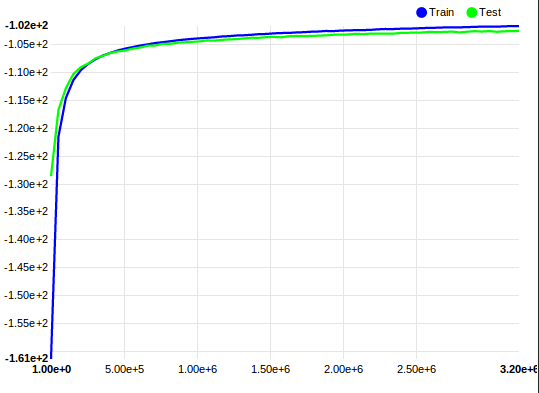
\includegraphics[scale=0.8,trim=0cm 0cm 0.1cm 0cm, clip=true]{images/MNIST_28_conv_nocuda.png}
	\caption{Lower bound for a one-layer DNN without subsampling trained on MNIST. A Spatial Convolution was also used in the Deconvolutional layer.}
	\label{label1}
\end{figure}

\subsubsection{2 layers}

\subsubsection{Overview}

Table \ref{overview} shows an overview of the results for MNIST experiments. 
\begin{table}
\caption{Overvieuw of results on MNIST. The Deconvolution Method row specifies which method, as described in Section 4.2, is used in the decoder.}
\renewcommand{\arraystretch}{1.5}
\label{overview}
\begin{tabular}{| l | l | l | l | l | l | l | l | l |}

	\hline
  Number of layers & 1 & 1 & 1 & 1 & 2 & 2 & 2 & .. \\ \hline
  Feature map size & 28 & 28 & 14 & 7 & .. & .. & .. & .. \\ \hline
  Deconvolution Method & Conv & MLP & MLP & MLP & .. & .. & .. & .. \\ \hline
  Total number of parameters & .. & .. & .. & .. & .. & .. & .. & .. \\ \hline
  Run time for one epoch with CUDA & .. & .. & .. & .. & .. & .. & .. & .. \\ \hline
  Train lower bound & 101,7 & .. & .. & .. & .. & .. & .. & .. \\ \hline
  Test lower bound & 102,57 & .. & .. & .. & .. & .. & .. & .. \\ \hline
  %1 & 28 	& SpatialConvolution 	& .. & .. & -.. \\ \hline
  %1 & 28 	& MLP					& .. & .. & -.. \\ \hline
  %1 & 14 	& MLP 					& .. & .. & -.. \\ \hline
  %1 & 7  	& MLP 					& .. & .. & -.. \\ \hline
  %2 & 14 14 	& SpatialConvolution 	& .. & .. & -.. \\ \hline
  %1 & 28 14	& SpatialConvolution 	& .. & .. & - N/A \\ \hline
  %1 & 14 7 	& SpatialConvolution 	& .. & .. & - N/A \\ \hline
\end{tabular}
\end{table}


\subsection{CIFAR-10}






%%%%%%%%%%%%%%%%%%%%%%%%%%%%%%%%%%%%%%%%%%
\begin{figure}
	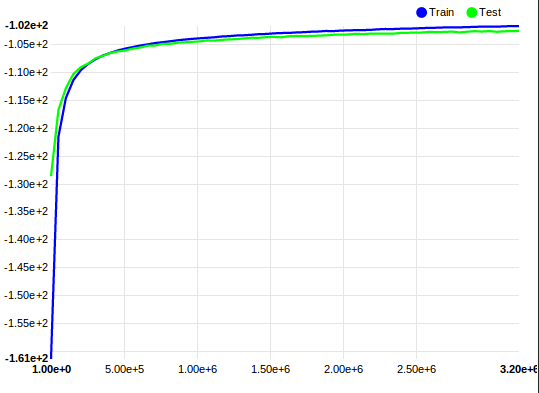
\includegraphics[scale=0.1]{images/MNIST_28_conv_nocuda.png}
	\caption{blablabla}
	\label{label1}
\end{figure}

\begin{figure}
	\centering
	\begin{subfigure}[b]{0.3\textwidth}		
		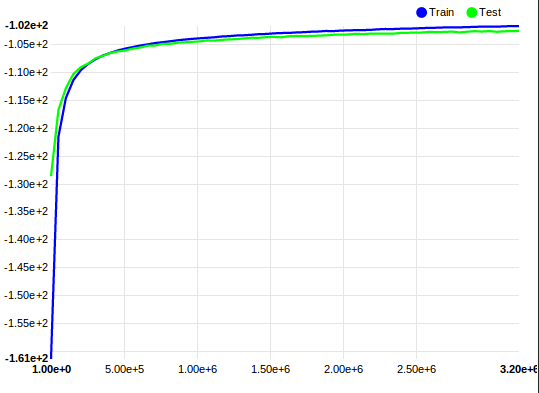
\includegraphics[scale=0.1]{images/MNIST_28_conv_nocuda.png}
		\caption{blablabla}
	\end{subfigure}

	\begin{subfigure}[b]{0.3\textwidth}		
		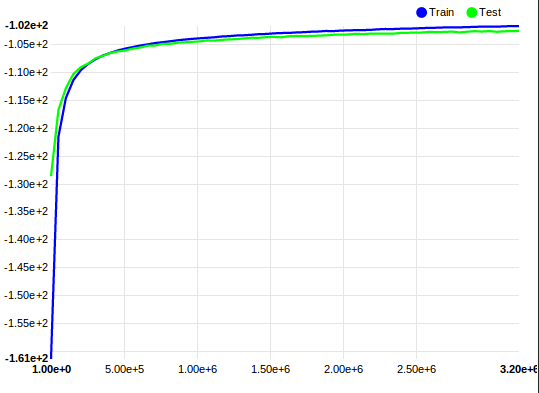
\includegraphics[scale=0.1]{images/MNIST_28_conv_nocuda.png}
		\caption{blablabla}
	\end{subfigure}
	\label{label2}
\end{figure}
\newpage


